\documentclass[aspectratio=169,usenames,dvipsnames,pdftex]{beamer}

\usepackage{listings}
\usepackage{xcolor}
\usepackage{multicol}
\usepackage{media9}
\usepackage{siunitx}
\usepackage[scale=2]{ccicons}
\usepackage{tabularx}
\usepackage{lmodern}
\usepackage{anyfontsize}

% Glyphs
\usepackage{fontawesome5}

\usepackage{booktabs}
\usepackage{appendixnumberbeamer}
\usepackage{csquotes}

\usepackage{pgfplots}
\usepgfplotslibrary{dateplot}

\usepackage{tikz}
\usetikzlibrary[topaths]
\usepackage{xspace}

\usetikzlibrary{shapes,snakes}
\usepackage{amsmath,amssymb}

%%%%%%%%%%%%%%%%
%% Title Page %%
%%%%%%%%%%%%%%%%
\title{Decentralized Vault (graduation project)}
\subtitle{\texttt{A Blockchain-based Decentralized Cloud Storage}}
\date {}
\author {
  \texttt{Supervisor:} \\
  \texttt{\large{Dr. Abdurrahman Nasr}} \\
  \\
  \texttt{Participants:} \\
  \texttt{\large{Abd El-Twab M. Fakhry}} \\
  \texttt{\large{Hossam Ahmed Elsaied Eissa}}
}
\institute {
  \centering
  Al-Azhar University \\
  Faculty of Engineering \\
  Computers \& Systems Engineering Department \\\vspace{8pt}
  \today
}

% \titlegraphic{\hfill\includegraphics[height=1.5cm]{}}

%%%%%%%%%%%%%%%%%%%
%% Common colors %%
%%%%%%%%%%%%%%%%%%%
\definecolor{charcoal}{rgb}{0.21, 0.27, 0.31}
\definecolor{champagne}{rgb}{0.97, 0.91, 0.81}
\definecolor{dimgray}{rgb}{0.41, 0.41, 0.41}
\definecolor{flax}{rgb}{0.93, 0.86, 0.51}
%% Code colors
\definecolor{lavendergray}{rgb}{0.77, 0.76, 0.82}
\definecolor{lightslategray}{rgb}{0.47, 0.53, 0.6}
\definecolor{egyptianblue}{rgb}{0.06, 0.2, 0.65}
\definecolor{ballblue}{rgb}{0.13, 0.67, 0.8}
\definecolor{greencssgreen}{rgb}{0.0, 0.5, 0.0}
\definecolor{eggshell}{rgb}{0.94, 0.92, 0.84}
\definecolor{lava}{rgb}{0.81, 0.06, 0.13}
\definecolor{lavenderindigo}{rgb}{0.58, 0.34, 0.92}
\definecolor{mediumred-violet}{rgb}{0.73, 0.2, 0.52}
\definecolor{black}{rgb}{0.0, 0.0, 0.0}
\definecolor{forestgreen}{rgb}{0.13, 0.55, 0.13}
\definecolor{harvardcrimson}{rgb}{0.79, 0.0, 0.09}

%%%%%%%%%%%%%%%%%%%%%%%%%
%% Syntax Highlighting %%
%%%%%%%%%%%%%%%%%%%%%%%%%
\lstdefinestyle{shared} {
  tabsize=2,
	showtabs=false,
	keepspaces=true,
  breaklines=true,
  showspaces=false,
  showstringspaces=false,
	breakatwhitespace=false,
  belowcaptionskip=1\baselineskip,
	captionpos=b,
  xleftmargin=\parindent,
	basicstyle=\ttfamily\footnotesize,
  numbers=left,
  numbersep=6pt,
	numberstyle=\tiny\color{lavenderindigo},
}

\lstdefinestyle{c}{
	language=C,
  style=shared,
	backgroundcolor=\color{eggshell},
	keywordstyle=\bfseries\color{egyptianblue},
	commentstyle=\itshape\color{lava},
  morecomment=[s][\color{forestgreen}]{/*+}{*/},
  morecomment=[s][\color{harvardcrimson}]{/*-}{*/},
	stringstyle=\color{greencssgreen},
	numberstyle=\tiny\color{lavenderindigo},
  % identifierstyle=\color{black},
  otherkeywords={size, printf, scanf, sizeof, memset},
  alsoletter = {\#},
  keywords=[2]{\#if,\#endif,\#else},
}

\lstdefinestyle{cpp} {
  language=C++,
  style=shared,
	backgroundcolor=\color{eggshell},
	keywordstyle=\bfseries\color{egyptianblue},
	commentstyle=\itshape\color{lava},
  morecomment=[s][\color{forestgreen}]{/*+}{*/},
  morecomment=[s][\color{harvardcrimson}]{/*-}{*/},
	stringstyle=\color{greencssgreen},
	numberstyle=\tiny\color{lavenderindigo},
  % identifierstyle=\color{black},
  otherkeywords={size, front, back, cin, cout, endl, sizeof, memset},
  alsoletter = {\#},
  keywords=[2]{\#if,\#endif,\#else},
}

\lstdefinelanguage{solidity} {
  morekeywords={pragma, contract, address, uint, bool, event, public,
    payable, constructor, function, require, for, if, emit, return,
    true, false, memory, storage},
  sensitive=true,
  morecomment=[l]{//},
  morecomment=[s]{/*}{*/},
  morecomment=[s][\color{forestgreen}]{/*+}{*/},
  morecomment=[s][\color{harvardcrimson}]{/*-}{*/},
  morestring=[b]",
  morestring=[b]'
}

\lstdefinestyle{solidity} {
  style=shared,
  language=solidity,
	backgroundcolor=\color{eggshell},
	keywordstyle=\bfseries\color{egyptianblue},
	commentstyle=\itshape\color{lava},
	stringstyle=\color{greencssgreen},
	numberstyle=\tiny\color{lavenderindigo},
  % identifierstyle=\color{black},
  otherkeywords={},
}

%%%%%%%%%%%
%% Theme %%
%%%%%%%%%%%
\usetheme[
progressbar=frametitle,
titleformat=smallcaps,
numbering=fraction,
block=fill,
background=light
]{metropolis}

\useoutertheme{metropolis}
\useinnertheme{metropolis}
\usefonttheme{metropolis}
\usecolortheme{seahorse}
\setbeamercolor{background canvas}{bg=champagne}
\setbeamercovered{transparent=5}

%%%%%%%%%%%%%%%%%%%%%%
%% Global Variables %%
%%%%%%%%%%%%%%%%%%%%%%
\newcommand{\themename}{\textbf{\textsc{Metropolis}}\xspace}
\newcount\mycount

%%%%%%%%%%%%%%%%%%%%
%% Document Start %%
%%%%%%%%%%%%%%%%%%%%
\begin{document}

	\maketitle

	\begin{frame}{Table of contents}
		\setbeamertemplate{section in toc}[sections numbered]
		\tableofcontents[hideallsubsections]
	\end{frame}

  \section{{Introduction}}

  \begin{frame}[t]{Background}\vspace{8pt}
    In the age of Big Data, The Internet Of Things, Digitization of every business, Data has become the biggest valuable asset for anyone.
    And it’s justly necessary to store it in an organized way such that it’s easily accessible and secure. \\[4pt]
    There are different ways to store data, such as local hard drives, flash memories, SD Cards, \textcolor{magenta}{\faCloud{}  cloud storage services}, and dare we even say DVDs? \\[10pt]

    \begin{block}{What is \faCloud{} cloud storage?}
      Cloud storage is a way to save data securely online so that it can be accessed anytime from any location and easily shared with those who are granted permission.
      It is usually accessed through an applications that use the API, such as cloud desktop storage, a cloud storage gateway or Web-based content management systems.
    \end{block}

  \end{frame}

  \begin{frame}[t]{Problem Statement}%\vspace{12pt}
    \begin{itemize}
    \item \texttt{\textcolor{red}{\faTimesCircle} Lack of Security and Privacy of Data} \\
      If your data is left unencrypted, any system administrator that has root privileges can see your content.
      Usually, companies look forward to your data so they can sell your data to other companies, suggest advertisements based on your data contents, and use it for their analysis.
    \item \texttt{\textcolor{red}{\faTimesCircle} Data Hack} \\
      It's not recommended to store your sensitive data on a centralized server that is financially profitable to get hacked.
    \item \texttt{\textcolor{red}{\faTimesCircle} Data Loss} \\
      Of course, you can always stick with local storage, But once they are lost, stolen, or most likely encrypted by ransomware, you cannot make a recovery.
    \end{itemize}
  \end{frame}

  \begin{frame}{Proposed Solution}
    The solution we propose for such a problem is to use:
    \begin{itemize}
    \item \textcolor{green}{\faCheckCircle{}} A distributed database system that will store data in a peer-to-peer network where is no central authority with the right to modify or censor clients' data.
    \item \textcolor{green}{\faCheckCircle{}} Encryption, so that everything should be encrypted before being uploaded.
    \item \textcolor{green}{\faCheckCircle{}} Diffusion, so that each object is shredded into small chunks. And object chunks are stored on different Nodes around the globe.
    \item \textcolor{green}{\faCheckCircle{}} A Blockchain and smart contract for managing data integrity and trust.
    \end{itemize}
  \end{frame}

  \begin{frame}{Related Theory}
    \begin{itemize}
    \item Public and Private Key Pairs
    \item Shamir’s secret sharing Algorithm
    \item Hashing
    \item Blockchain
    \end{itemize}
  \end{frame}

  \section{Methodology}

  \begin{frame}{Peer to Peer Network}
    Instead of establishing a new peer-to-peer Network, we are using IPFS Protocol.
    \begin{block}{What is the IPFS?}
      \texttt{IPFS,} The Interplanetary File System is a distributed system for storing and accessing files, applications, and websites. It is a worldwide peer-to-peer file-sharing system created by Protocol Labs.  It is inspired by good ideas from BitTorrent, Git, and Kademlia.
    \end{block}
  \end{frame}

  \section{Development Methodology}

  \begin{frame}{Software Development Approach}
    We have chosen the Scrum methodology. It’s a popular way to implement agile, and it allows the team to deliver software regularly
    \begin{figure}
      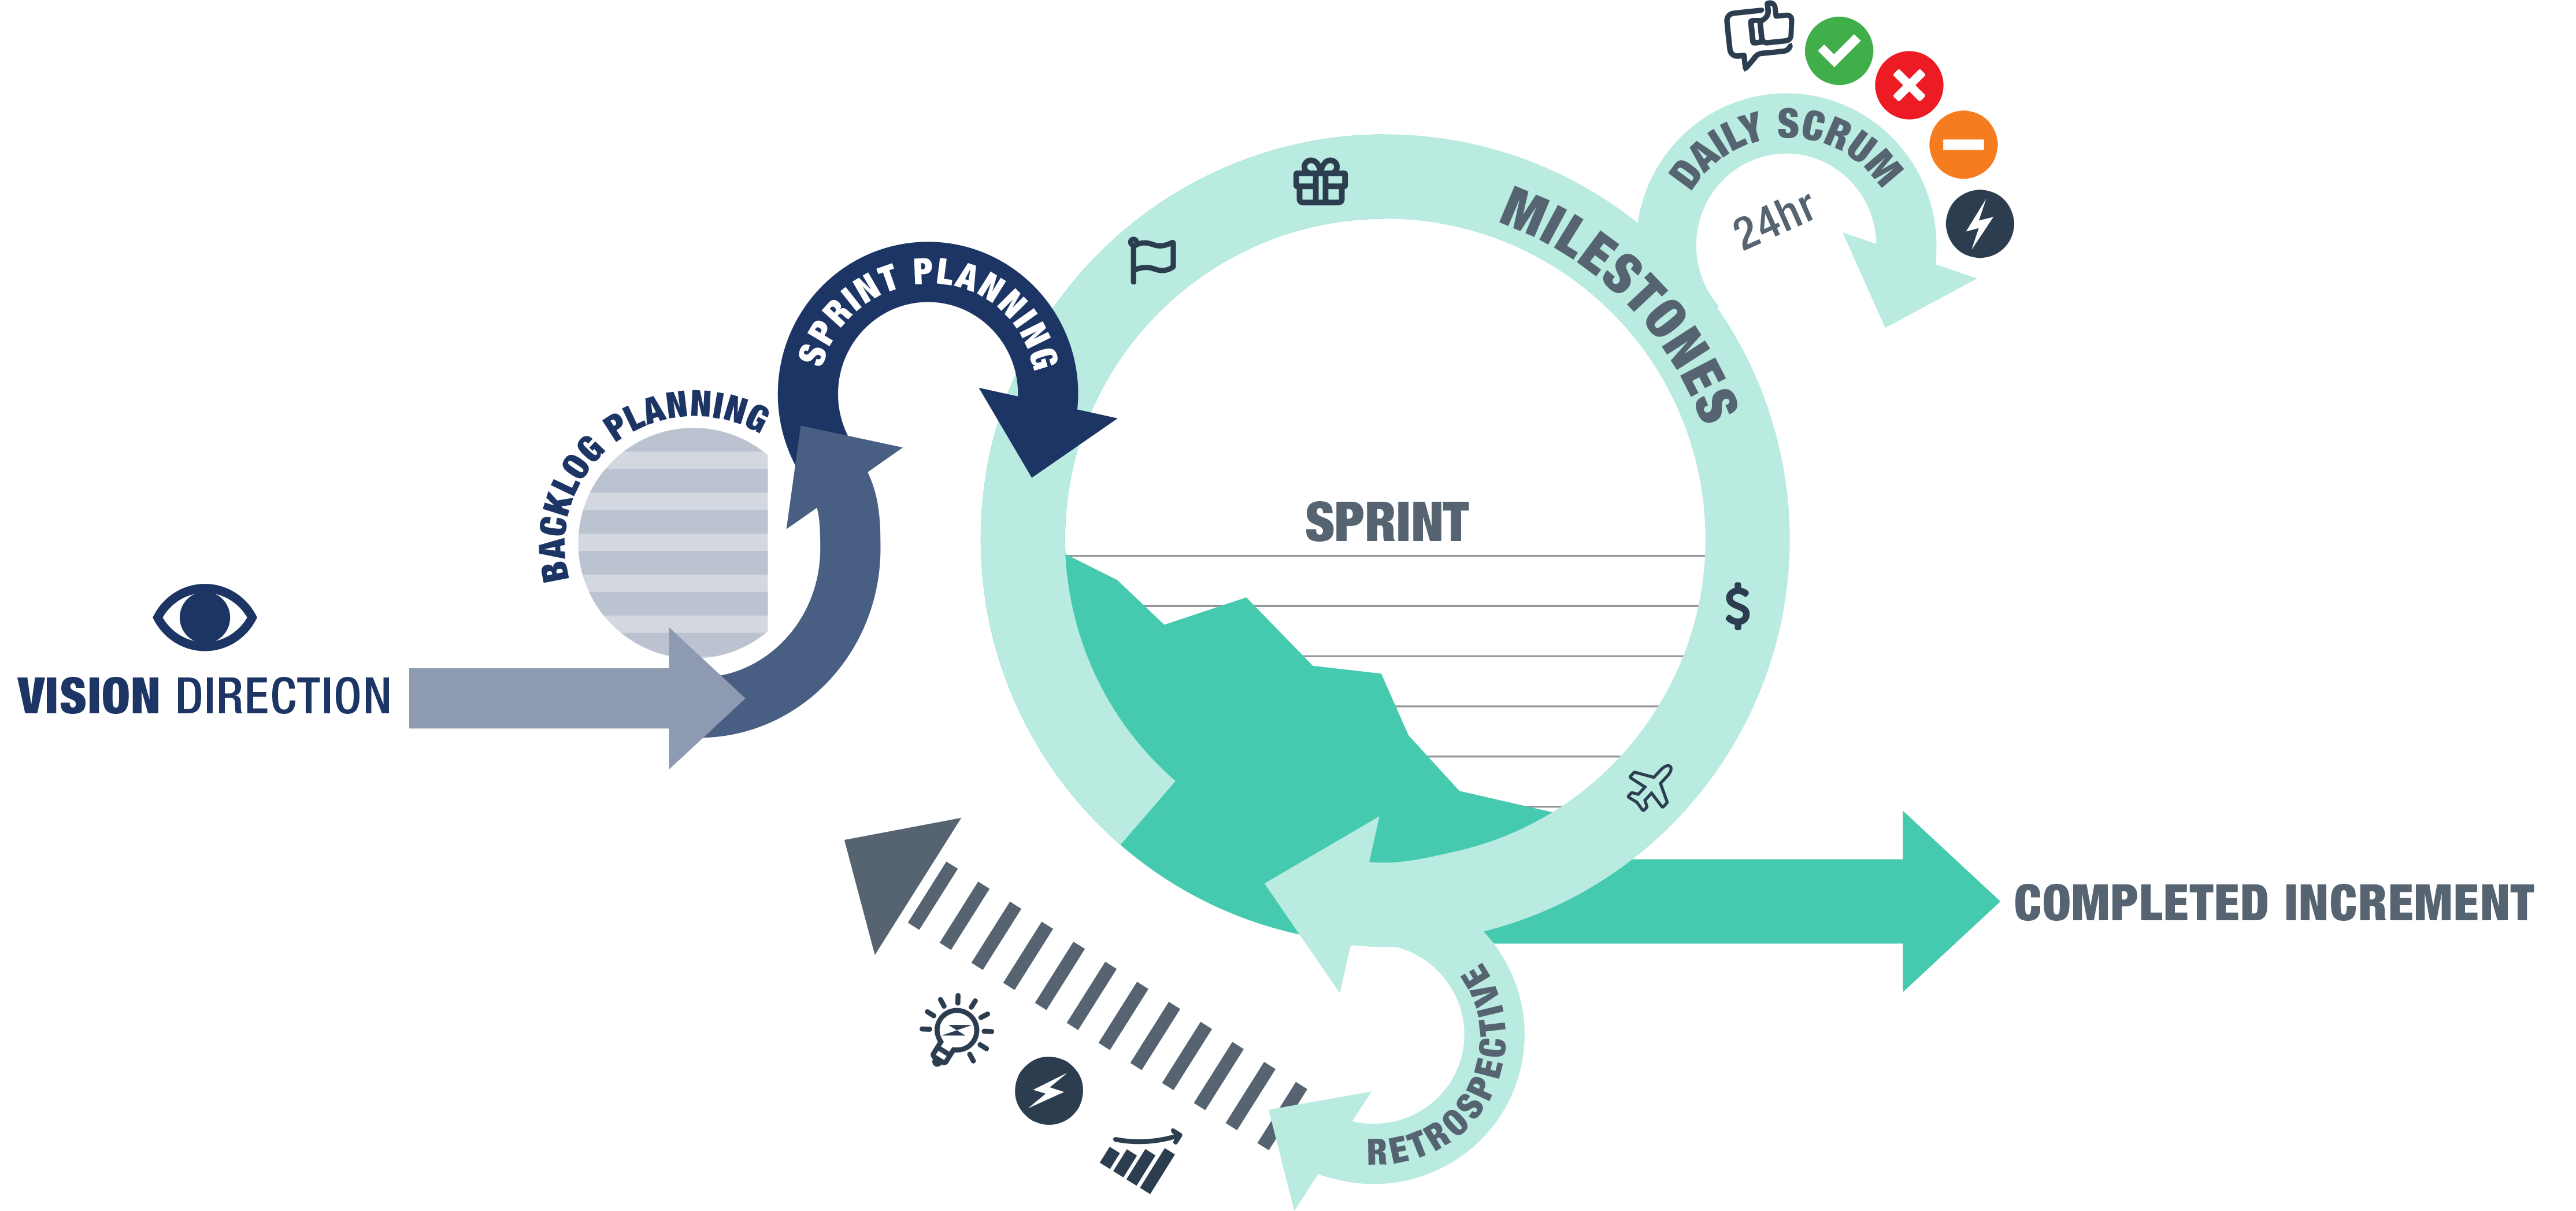
\includegraphics[width=0.8\textwidth]{agile-scrum.png}
      \caption{Scrum Methodology}
    \end{figure}
  \end{frame}

  \begin{frame}{Tools and Technologies}
    \begin{itemize}
      \begin{multicols}{2}
      \item \faNode{} Node.js
      \item Solidity (Smart contract)
      \item \faCodeBranch{} Github Actions (CI/CD)
      \item Mocha (Unit test)
      \item Rinkeby (Test net)
      \item \faGitSquare{} Git (Version control)
      \item \faJira{} Jira (Issue tracking)
      \item \faReact{} Next.js (React.js framework)
      \item Hardhat (Solidity framework)
      \item \faDocker{} Docker (Deployment)
      \item ESLint (Linting code base)
      \item Ethers (Library)
      \item \faGithub{} Github (Remote repository)
      \item Infura (IPFS gateway)
      \end{multicols}
    \end{itemize}
  \end{frame}

  \begin{frame}{Project Diagram}
    \begin{figure}
      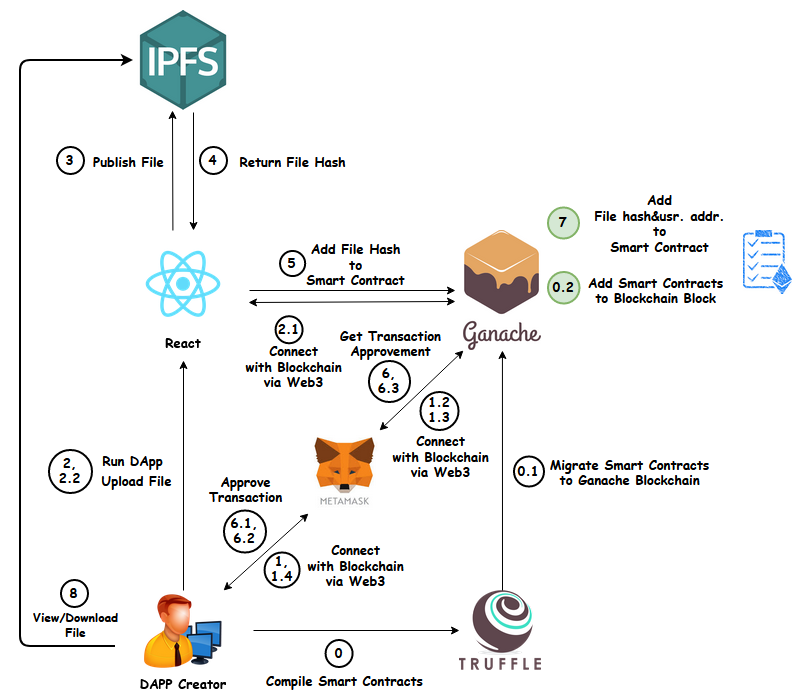
\includegraphics[width=0.53\textwidth]{system-diagram.png}
      \caption{Project Diagram}
    \end{figure}
  \end{frame}

  \begin{frame}{Usecase UML Diagram}
    \begin{figure}
      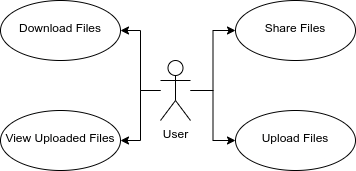
\includegraphics[width=0.5\textwidth]{usecase-uml.png}
      \caption{Usecase UML Diagram}
    \end{figure}
  \end{frame}

	\section{Conclusion}

	\begin{frame}{Summary}
    \begin{quote}
      You deserve to live a sustainable, private, self-sufficient and independent life, don't let anyone take this from you.
    \end{quote}
	\end{frame}

	\begin{frame}[standout]
		Thanks!
	\end{frame}

  % \appendix

	\begin{frame}[allowframebreaks]{References}
    \nocite{*}
    \bibliography{biblio}
		\bibliographystyle{unsrt}
	\end{frame}

\end{document}
